\renewcommand{\theequation}{\theenumi}
\begin{enumerate}[label=\arabic*.,ref=\thesubsubsection.\theenumi]
\numberwithin{equation}{enumi}
%
\item Let the boy be at point $\vec{B}=\myvec{0\\0}$
\\
Initially, it was initially raining downward at speed of 35 $m s^{-1}$ and when there is wind, it is raining downward at speed of 12 $m s^{-1}$.
The angle $\theta$ with the vertical, at which it is raining is calculated by:
\begin{align}
35 \cos\theta=\frac{12}{35}
\\
\implies \theta=69.94^{\circ}
\end{align}  
$\therefore$ Boy has to hold his umbrella at angle of $20 ^{\circ}$ with the ground towards east.
\\
The code for the diagramatic(\ref{fig:speed}) representation of the solution is
\begin{lstlisting}
codes/line/speed.py
\end{lstlisting}
\begin{figure}[!ht]
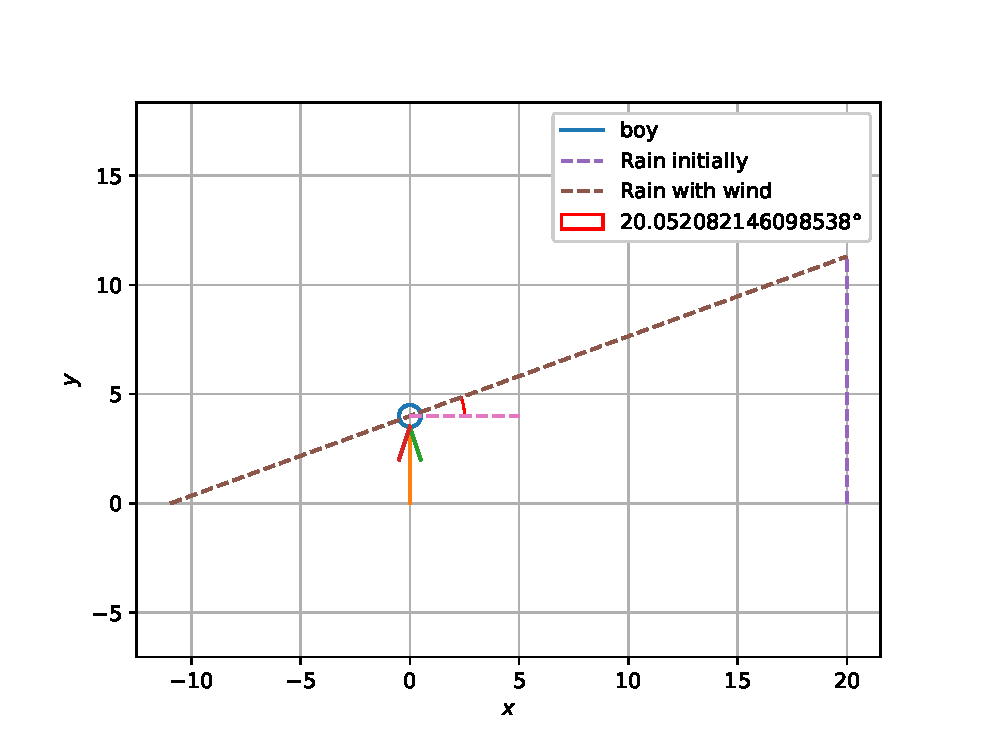
\includegraphics[width=\columnwidth]{./figs/line/speed.eps}
\caption{}
\label{fig:speed}
\end{figure}
\end{enumerate}
